\documentclass[10pt,a4paper,draft]{article}
\usepackage[utf8x]{inputenc}
\usepackage{ucs}
\usepackage[english]{babel}
\usepackage{multirow}
\usepackage{rotating}
\author{Lukáš Petrovický}
\title{RAS2012: Competition Entry}
\begin{document}

\maketitle

\begin{abstract}
This article describes an entry to the 2012 RAS Problem Solving Competition, concerning dispatching on multi-track territories. The entry is based on the Drools Planner, a Java-based solver. On a reasonably recent computer, the resulting algorithm is able to produce feasible results within a minute and has been fine-tuned to provide best results in under 3 minutes. Source code to the entry is open source and well documented.
\end{abstract}

\section{Introduction}

\section{Describing the solution}

\section{Implementation}

\section{Conclusion}

\appendix

\section{Resolved systems}

In this section, we show the best solutions reached for each data set. All these were reached within 3 minutes in a single-threaded run, using Intel i7 Q820 processor running Fedora 17 and 1 GB of heap space inside Java 7 runtime environment. Please note that via the benchmarking functionality of Drools planner (see above), users may be able to fine-tune the algorithm. This fine-tuning can be focused either on providing better solutions or on faster turnaround times.

\begin{sidewaystable}
\footnotesize
\caption{Statistics for resolved system ``RAS DATA SET 1'', costing \$1584.}
\centering
\begin{tabular}{c||c|c||c|c|c|c|c||c|c|c}
  \hline \hline
  &
  Unpref. & 
  Delay &
  Node &
  When &
  SA &
  +/- &
  Pty &
  TWT &
  +/- &
  Pty \\
      \hline
      \multirow{2}{*}{A1} &
      \multirow{2}{*}{0} &
      \multirow{2}{*}{0} &
      37 &
      3469.5 &
      3600 &
        130.5 &
        0 &
      \multirow{2}{*}{5400} &
        \multirow{2}{*}{-1003.5} &
        \multirow{2}{*}{0}
      \\
      \cline{4-8}
       &
       &
       &
      39 &
      6403.5 &
      7800 &
        1396.5 &
        0 &
      
         &
        
      \\
      \hline
      \multirow{2}{*}{A2} &
      \multirow{2}{*}{27} &
      \multirow{2}{*}{1620} &
      37 &
      6184.742 &
      7800 &
        1615.258 &
        0 &
      \multirow{2}{*}{9000} &
        \multirow{2}{*}{-1509.166} &
        \multirow{2}{*}{0}
      \\
      \cline{4-8}
       &
       &
       &
      39 &
      10509.166 &
      12000 &
        1490.834 &
        0 &
      
         &
        
      \\
      \hline
      \multirow{2}{*}{B1} &
      \multirow{2}{*}{11} &
      \multirow{2}{*}{0} &
      37 &
      10486.282 &
      12600 &
        2113.718 &
        0 &
      \multirow{2}{*}{13800} &
        \multirow{2}{*}{-63.266} &
        \multirow{2}{*}{0}
      \\
      \cline{4-8}
       &
       &
       &
      0 &
      13863.266 &
      17400 &
        3536.734 &
        0 &
      
         &
        
      \\
      \hline
      \multirow{2}{*}{B2} &
      \multirow{2}{*}{0} &
      \multirow{2}{*}{1920} &
      37 &
      13621.758 &
      15600 &
        1978.242 &
        0 &
      \multirow{2}{*}{16800} &
        \multirow{2}{*}{-2091.87} &
        \multirow{2}{*}{0}
      \\
      \cline{4-8}
       &
       &
       &
      39 &
      18891.87 &
      19800 &
        908.13 &
        0 &
      
         &
        
      \\
      \hline
      \multirow{2}{*}{B3} &
      \multirow{2}{*}{14} &
      \multirow{2}{*}{2520} &
      37 &
      41125.571 &
      40200 &
        -925.571 &
        0 &
      \multirow{2}{*}{42000} &
        \multicolumn{2}{c}{\multirow{2}{*}{N/A}}
      \\
      \cline{4-8}
       &
       &
       &
      39 &
      44099.393 &
      45000 &
        \multicolumn{2}{|c||}{N/A} &
      
        
      \\
      \hline
      \multirow{2}{*}{C1} &
      \multirow{2}{*}{0} &
      \multirow{2}{*}{0} &
      37 &
      17946 &
      19200 &
        1254 &
        0 &
      \multirow{2}{*}{21600} &
        \multirow{2}{*}{282} &
        \multirow{2}{*}{0}
      \\
      \cline{4-8}
       &
       &
       &
      39 &
      21318 &
      24600 &
        3282 &
        0 &
      
         &
        
      \\
      \hline
      \multirow{2}{*}{C2} &
      \multirow{2}{*}{0} &
      \multirow{2}{*}{0} &
      37 &
      25026.431 &
      27000 &
        1973.569 &
        0 &
      \multirow{2}{*}{28800} &
        \multirow{2}{*}{165.853} &
        \multirow{2}{*}{0}
      \\
      \cline{4-8}
       &
       &
       &
      39 &
      28634.147 &
      33000 &
        4365.853 &
        0 &
      
         &
        
      \\
      \hline
      \multirow{2}{*}{D1} &
      \multirow{2}{*}{0} &
      \multirow{2}{*}{0} &
      37 &
      26334.852 &
      29400 &
        3065.148 &
        0 &
      \multirow{2}{*}{31200} &
        \multirow{2}{*}{296.584} &
        \multirow{2}{*}{0}
      \\
      \cline{4-8}
       &
       &
       &
      0 &
      30903.416 &
      36600 &
        5696.584 &
        0 &
      
         &
        
      \\
      \hline
      \multirow{2}{*}{D2} &
      \multirow{2}{*}{15} &
      \multirow{2}{*}{1920} &
      37 &
      20743.649 &
      21600 &
        856.351 &
        0 &
      \multirow{2}{*}{23400} &
        \multirow{2}{*}{-2067.362} &
        \multirow{2}{*}{0}
      \\
      \cline{4-8}
       &
       &
       &
      0 &
      25467.362 &
      28200 &
        2732.638 &
        0 &
      
         &
        
      \\
      \hline
      \multirow{2}{*}{D3} &
      \multirow{2}{*}{0} &
      \multirow{2}{*}{0} &
      37 &
      33181.717 &
      35400 &
        2218.283 &
        0 &
      \multirow{2}{*}{37200} &
        \multirow{2}{*}{-433.597} &
        \multirow{2}{*}{0}
      \\
      \cline{4-8}
       &
       &
       &
      0 &
      37633.597 &
      41400 &
        3766.403 &
        0 &
      
         &
        
      \\
      \hline
      \multirow{2}{*}{E1} &
      \multirow{2}{*}{0} &
      \multirow{2}{*}{11340} &
      37 &
      54507 &
      36000 &
        \multicolumn{2}{|c||}{N/A} &
      \multirow{2}{*}{39000} &
        \multicolumn{2}{c}{\multirow{2}{*}{N/A}}
      \\
      \cline{4-8}
       &
       &
       &
      39 &
      59925 &
      44400 &
        \multicolumn{2}{|c||}{N/A} &
      
        
      \\
      \hline
      \multirow{2}{*}{F1} &
      \multirow{2}{*}{0} &
      \multirow{2}{*}{0} &
      37 &
      51006.856 &
      57600 &
        \multicolumn{2}{|c||}{N/A} &
      \multirow{2}{*}{63000} &
        \multicolumn{2}{c}{\multirow{2}{*}{N/A}}
      \\
      \cline{4-8}
       &
       &
       &
      0 &
      61971.425 &
      75000 &
        \multicolumn{2}{|c||}{N/A} &
      
        
      \\
\end{tabular}
\label{table:RDS1-1584.tex} 
\end{sidewaystable}
\begin{sidewaystable}
\footnotesize
\caption{Statistics for resolved system ``RAS DATA SET 2'', costing \$9235.}
\centering
\begin{tabular}{c||c|c||c|c|c|c|c||c|c|c}
  \hline \hline
  &
  Unpref. & 
  Delay &
  Node &
  When &
  SA &
  +/- &
  Pty &
  TWT &
  +/- &
  Pty \\
      \hline
      \multirow{2}{*}{A1} &
      \multirow{2}{*}{4} &
      \multirow{2}{*}{2760} &
      37 &
      5842.5 &
      3600 &
        -2242.5 &
        0 &
      \multirow{2}{*}{5400} &
        \multirow{2}{*}{-3880.5} &
        \multirow{2}{*}{0}
      \\
      \cline{4-8}
       &
       &
       &
      39 &
      9280.5 &
      7800 &
        -1480.5 &
        0 &
      
         &
        
      \\
      \hline
      \multirow{2}{*}{A2} &
      \multirow{2}{*}{0} &
      \multirow{2}{*}{240} &
      37 &
      10636.424 &
      11400 &
        763.576 &
        0 &
      \multirow{2}{*}{12600} &
        \multirow{2}{*}{-713.692} &
        \multirow{2}{*}{0}
      \\
      \cline{4-8}
       &
       &
       &
      39 &
      13313.692 &
      15600 &
        2286.308 &
        0 &
      
         &
        
      \\
      \hline
      \multirow{2}{*}{A3} &
      \multirow{2}{*}{4} &
      \multirow{2}{*}{0} &
      37 &
      17095.5 &
      18000 &
        904.5 &
        0 &
      \multirow{2}{*}{19800} &
        \multirow{2}{*}{-346.5} &
        \multirow{2}{*}{0}
      \\
      \cline{4-8}
       &
       &
       &
      39 &
      20146.5 &
      22200 &
        2053.5 &
        0 &
      
         &
        
      \\
      \hline
      \multirow{2}{*}{A4} &
      \multirow{2}{*}{22} &
      \multirow{2}{*}{60} &
      37 &
      36347.461 &
      31800 &
        -4547.461 &
        0 &
      \multirow{2}{*}{39000} &
        \multirow{2}{*}{-959.375} &
        \multirow{2}{*}{0}
      \\
      \cline{4-8}
       &
       &
       &
      0 &
      39959.375 &
      36600 &
        -3359.375 &
        0 &
      
         &
        
      \\
      \hline
      \multirow{2}{*}{B1} &
      \multirow{2}{*}{9} &
      \multirow{2}{*}{7260} &
      37 &
      14048.112 &
      4800 &
        -9248.112 &
        113 &
      \multirow{2}{*}{9600} &
        \multirow{2}{*}{-7798.224} &
        \multirow{2}{*}{0}
      \\
      \cline{4-8}
       &
       &
       &
      39 &
      17398.224 &
      9000 &
        -8398.224 &
        66 &
      
         &
        
      \\
      \hline
      \multirow{2}{*}{B2} &
      \multirow{2}{*}{16} &
      \multirow{2}{*}{120} &
      37 &
      32423.625 &
      26400 &
        -6023.625 &
        0 &
      \multirow{2}{*}{35400} &
        \multirow{2}{*}{-777.375} &
        \multirow{2}{*}{0}
      \\
      \cline{4-8}
       &
       &
       &
      39 &
      36177.375 &
      31200 &
        -4977.375 &
        0 &
      
         &
        
      \\
      \hline
      \multirow{2}{*}{B3} &
      \multirow{2}{*}{8} &
      \multirow{2}{*}{0} &
      37 &
      7313.144 &
      11400 &
        4086.856 &
        0 &
      \multirow{2}{*}{10800} &
        \multirow{2}{*}{60.425} &
        \multirow{2}{*}{0}
      \\
      \cline{4-8}
       &
       &
       &
      0 &
      10739.575 &
      16800 &
        6060.425 &
        0 &
      
         &
        
      \\
      \hline
      \multirow{2}{*}{C1} &
      \multirow{2}{*}{0} &
      \multirow{2}{*}{60} &
      37 &
      35829.006 &
      26400 &
        -9429.006 &
        123 &
      \multirow{2}{*}{39000} &
        \multirow{2}{*}{-134.089} &
        \multirow{2}{*}{0}
      \\
      \cline{4-8}
       &
       &
       &
      39 &
      39134.089 &
      31800 &
        -7334.089 &
        7 &
      
         &
        
      \\
      \hline
      \multirow{2}{*}{C2} &
      \multirow{2}{*}{0} &
      \multirow{2}{*}{0} &
      37 &
      198 &
      0 &
        -198 &
        0 &
      \multirow{2}{*}{3600} &
        \multirow{2}{*}{30} &
        \multirow{2}{*}{0}
      \\
      \cline{4-8}
       &
       &
       &
      39 &
      3570 &
      5400 &
        1830 &
        0 &
      
         &
        
      \\
      \hline
      \multirow{2}{*}{C3} &
      \multirow{2}{*}{0} &
      \multirow{2}{*}{22433.141} &
      37 &
      59181.43 &
      20400 &
        \multicolumn{2}{|c||}{N/A} &
      \multirow{2}{*}{25200} &
        \multicolumn{2}{c}{\multirow{2}{*}{N/A}}
      \\
      \cline{4-8}
       &
       &
       &
      0 &
      63784.718 &
      25800 &
        \multicolumn{2}{|c||}{N/A} &
      
        
      \\
      \hline
      \multirow{2}{*}{D1} &
      \multirow{2}{*}{0} &
      \multirow{2}{*}{0} &
      37 &
      40216.5 &
      43800 &
        3583.5 &
        0 &
      \multirow{2}{*}{44400} &
        \multicolumn{2}{c}{\multirow{2}{*}{N/A}}
      \\
      \cline{4-8}
       &
       &
       &
      39 &
      44722.5 &
      51000 &
        \multicolumn{2}{|c||}{N/A} &
      
        
      \\
      \hline
      \multirow{2}{*}{D2} &
      \multirow{2}{*}{27} &
      \multirow{2}{*}{1800} &
      37 &
      2179.383 &
      3600 &
        1420.617 &
        0 &
      \multirow{2}{*}{6600} &
        \multirow{2}{*}{-1361.531} &
        \multirow{2}{*}{0}
      \\
      \cline{4-8}
       &
       &
       &
      39 &
      7961.531 &
      9600 &
        1638.469 &
        0 &
      
         &
        
      \\
      \hline
      \multirow{2}{*}{E1} &
      \multirow{2}{*}{0} &
      \multirow{2}{*}{43200} &
      37 &
      48820.912 &
      6600 &
        \multicolumn{2}{|c||}{N/A} &
      \multirow{2}{*}{9600} &
        \multicolumn{2}{c}{\multirow{2}{*}{N/A}}
      \\
      \cline{4-8}
       &
       &
       &
      39 &
      54087.822 &
      14400 &
        \multicolumn{2}{|c||}{N/A} &
      
        
      \\
      \hline
      \multirow{2}{*}{E2} &
      \multirow{2}{*}{0} &
      \multirow{2}{*}{0} &
      37 &
      1134.858 &
      1800 &
        665.142 &
        0 &
      \multirow{2}{*}{7200} &
        \multirow{2}{*}{-26.294} &
        \multirow{2}{*}{0}
      \\
      \cline{4-8}
       &
       &
       &
      0 &
      7226.294 &
      10800 &
        3573.706 &
        0 &
      
         &
        
      \\
      \hline
      \multirow{2}{*}{E3} &
      \multirow{2}{*}{0} &
      \multirow{2}{*}{43200} &
      37 &
      97546.285 &
      9000 &
        \multicolumn{2}{|c||}{N/A} &
      \multirow{2}{*}{12000} &
        \multicolumn{2}{c}{\multirow{2}{*}{N/A}}
      \\
      \cline{4-8}
       &
       &
       &
      0 &
      105575.14 &
      18000 &
        \multicolumn{2}{|c||}{N/A} &
      
        
      \\
      \hline
      \multirow{2}{*}{E4} &
      \multirow{2}{*}{32} &
      \multirow{2}{*}{0} &
      37 &
      27424.521 &
      30000 &
        2575.479 &
        0 &
      \multirow{2}{*}{32400} &
        \multirow{2}{*}{-269.3} &
        \multirow{2}{*}{0}
      \\
      \cline{4-8}
       &
       &
       &
      0 &
      32669.3 &
      37800 &
        5130.7 &
        0 &
      
         &
        
      \\
      \hline
      \multirow{2}{*}{F1} &
      \multirow{2}{*}{39} &
      \multirow{2}{*}{840} &
      37 &
      25268.18 &
      29400 &
        4131.82 &
        0 &
      \multirow{2}{*}{33600} &
        \multirow{2}{*}{1.638} &
        \multirow{2}{*}{0}
      \\
      \cline{4-8}
       &
       &
       &
      39 &
      33598.362 &
      41400 &
        7801.638 &
        0 &
      
         &
        
      \\
      \hline
      \multirow{2}{*}{F2} &
      \multirow{2}{*}{0} &
      \multirow{2}{*}{34560} &
      37 &
      63080.573 &
      30000 &
        \multicolumn{2}{|c||}{N/A} &
      \multirow{2}{*}{36000} &
        \multicolumn{2}{c}{\multirow{2}{*}{N/A}}
      \\
      \cline{4-8}
       &
       &
       &
      0 &
      76786.29 &
      51000 &
        \multicolumn{2}{|c||}{N/A} &
      
        
      \\
\end{tabular}
\label{table:RDS2-9235.tex} 
\end{sidewaystable}
\begin{sidewaystable}
\footnotesize
\caption{Statistics for resolved system ``RAS DATA SET 3'', costing \$13338.}
\centering
\begin{tabular}{c||c|c||c|c|c|c|c||c|c|c}
  \hline \hline
  &
  Unpref. & 
  Delay &
  Node &
  When &
  SA &
  +/- &
  Pty &
  TWT &
  +/- &
  Pty \\
      \hline
      \multirow{2}{*}{A1} &
      \multirow{2}{*}{0} &
      \multirow{2}{*}{0} &
      37 &
      1354.5 &
      2400 &
        1045.5 &
        0 &
      \multirow{2}{*}{4200} &
        \multirow{2}{*}{298.5} &
        \multirow{2}{*}{0}
      \\
      \cline{4-8}
       &
       &
       &
      39 &
      3901.5 &
      6000 &
        2098.5 &
        0 &
      
         &
        
      \\
      \hline
      \multirow{2}{*}{A2} &
      \multirow{2}{*}{13} &
      \multirow{2}{*}{120} &
      37 &
      1560 &
      2400 &
        840 &
        0 &
      \multirow{2}{*}{4200} &
        \multirow{2}{*}{-841.718} &
        \multirow{2}{*}{0}
      \\
      \cline{4-8}
       &
       &
       &
      0 &
      5041.718 &
      6600 &
        1558.282 &
        0 &
      
         &
        
      \\
      \hline
      \multirow{2}{*}{A3} &
      \multirow{2}{*}{10} &
      \multirow{2}{*}{0} &
      37 &
      20900.576 &
      22800 &
        1899.424 &
        0 &
      \multirow{2}{*}{24000} &
        \multirow{2}{*}{-292.294} &
        \multirow{2}{*}{0}
      \\
      \cline{4-8}
       &
       &
       &
      0 &
      24292.294 &
      27000 &
        2707.706 &
        0 &
      
         &
        
      \\
      \hline
      \multirow{2}{*}{A4} &
      \multirow{2}{*}{15} &
      \multirow{2}{*}{0} &
      37 &
      36175.943 &
      33600 &
        -2575.943 &
        0 &
      \multirow{2}{*}{39000} &
        \multirow{2}{*}{-1061.104} &
        \multirow{2}{*}{0}
      \\
      \cline{4-8}
       &
       &
       &
      0 &
      40061.104 &
      38400 &
        -1661.104 &
        0 &
      
         &
        
      \\
      \hline
      \multirow{2}{*}{A5} &
      \multirow{2}{*}{0} &
      \multirow{2}{*}{4815} &
      37 &
      36697.5 &
      32400 &
        -4297.5 &
        0 &
      \multirow{2}{*}{34200} &
        \multirow{2}{*}{-5044.5} &
        \multirow{2}{*}{0}
      \\
      \cline{4-8}
       &
       &
       &
      39 &
      39244.5 &
      36600 &
        -2644.5 &
        0 &
      
         &
        
      \\
      \hline
      \multirow{1}{*}{B1} &
      \multirow{1}{*}{0} &
      \multirow{1}{*}{0} &
      0 &
      1486.284 &
      1800 &
        313.716 &
        0 &
      \multirow{1}{*}{1200} &
        \multirow{1}{*}{-286.284} &
        \multirow{1}{*}{0}
      \\
      \hline
      \multirow{1}{*}{B2} &
      \multirow{1}{*}{0} &
      \multirow{1}{*}{0} &
      39 &
      2869.163 &
      4800 &
        1930.837 &
        0 &
      \multirow{1}{*}{3000} &
        \multirow{1}{*}{130.837} &
        \multirow{1}{*}{0}
      \\
      \hline
      \multirow{2}{*}{B3} &
      \multirow{2}{*}{8} &
      \multirow{2}{*}{6180} &
      37 &
      9230.026 &
      -3000 &
        -12230.026 &
        279 &
      \multirow{2}{*}{6000} &
        \multirow{2}{*}{-7128.005} &
        \multirow{2}{*}{0}
      \\
      \cline{4-8}
       &
       &
       &
      39 &
      13128.005 &
      1800 &
        -11328.005 &
        229 &
      
         &
        
      \\
      \hline
      \multirow{2}{*}{B4} &
      \multirow{2}{*}{2} &
      \multirow{2}{*}{14460} &
      37 &
      43229.145 &
      16800 &
        \multicolumn{2}{|c||}{N/A} &
      \multirow{2}{*}{32400} &
        \multicolumn{2}{c}{\multirow{2}{*}{N/A}}
      \\
      \cline{4-8}
       &
       &
       &
      0 &
      46655.576 &
      21600 &
        \multicolumn{2}{|c||}{N/A} &
      
        
      \\
      \hline
      \multirow{1}{*}{C1} &
      \multirow{1}{*}{0} &
      \multirow{1}{*}{22140} &
      0 &
      25808.568 &
      6000 &
        -19808.568 &
        700 &
      \multirow{1}{*}{4200} &
        \multirow{1}{*}{-21608.568} &
        \multirow{1}{*}{225}
      \\
      \hline
      \multirow{2}{*}{C2} &
      \multirow{2}{*}{13} &
      \multirow{2}{*}{1140} &
      37 &
      5090.145 &
      0 &
        -5090.145 &
        0 &
      \multirow{2}{*}{7200} &
        \multirow{2}{*}{-1624.718} &
        \multirow{2}{*}{0}
      \\
      \cline{4-8}
       &
       &
       &
      39 &
      8824.718 &
      6000 &
        -2824.718 &
        0 &
      
         &
        
      \\
      \hline
      \multirow{2}{*}{C3} &
      \multirow{2}{*}{0} &
      \multirow{2}{*}{10550.201} &
      37 &
      47268.738 &
      30000 &
        \multicolumn{2}{|c||}{N/A} &
      \multirow{2}{*}{37200} &
        \multicolumn{2}{c}{\multirow{2}{*}{N/A}}
      \\
      \cline{4-8}
       &
       &
       &
      0 &
      51184.66 &
      36000 &
        \multicolumn{2}{|c||}{N/A} &
      
        
      \\
      \hline
      \multirow{2}{*}{D1} &
      \multirow{2}{*}{0} &
      \multirow{2}{*}{4740} &
      37 &
      8369.995 &
      4200 &
        -4169.995 &
        0 &
      \multirow{2}{*}{7800} &
        \multirow{2}{*}{-4509.681} &
        \multirow{2}{*}{0}
      \\
      \cline{4-8}
       &
       &
       &
      39 &
      12309.681 &
      10200 &
        -2109.681 &
        0 &
      
         &
        
      \\
      \hline
      \multirow{2}{*}{D2} &
      \multirow{2}{*}{0} &
      \multirow{2}{*}{0} &
      37 &
      40013.996 &
      42000 &
        1986.004 &
        0 &
      \multirow{2}{*}{43800} &
        \multicolumn{2}{c}{\multirow{2}{*}{N/A}}
      \\
      \cline{4-8}
       &
       &
       &
      39 &
      43893.682 &
      48000 &
        \multicolumn{2}{|c||}{N/A} &
      
        
      \\
      \hline
      \multirow{2}{*}{E1} &
      \multirow{2}{*}{0} &
      \multirow{2}{*}{43200} &
      37 &
      49849.148 &
      10200 &
        \multicolumn{2}{|c||}{N/A} &
      \multirow{2}{*}{13200} &
        \multicolumn{2}{c}{\multirow{2}{*}{N/A}}
      \\
      \cline{4-8}
       &
       &
       &
      0 &
      55940.584 &
      19200 &
        \multicolumn{2}{|c||}{N/A} &
      
        
      \\
      \hline
      \multirow{2}{*}{E2} &
      \multirow{2}{*}{35} &
      \multirow{2}{*}{4644} &
      37 &
      20487 &
      18000 &
        -2487 &
        0 &
      \multirow{2}{*}{21000} &
        \multirow{2}{*}{-4929} &
        \multirow{2}{*}{0}
      \\
      \cline{4-8}
       &
       &
       &
      39 &
      25929 &
      26400 &
        471 &
        0 &
      
         &
        
      \\
      \hline
      \multirow{2}{*}{E3} &
      \multirow{2}{*}{6} &
      \multirow{2}{*}{0} &
      37 &
      19052.184 &
      21000 &
        1947.816 &
        0 &
      \multirow{2}{*}{24000} &
        \multirow{2}{*}{-10.366} &
        \multirow{2}{*}{0}
      \\
      \cline{4-8}
       &
       &
       &
      39 &
      24010.366 &
      28800 &
        4789.634 &
        0 &
      
         &
        
      \\
      \hline
      \multirow{2}{*}{E4} &
      \multirow{2}{*}{0} &
      \multirow{2}{*}{9060} &
      37 &
      46790 &
      40800 &
        \multicolumn{2}{|c||}{N/A} &
      \multirow{2}{*}{43800} &
        \multicolumn{2}{c}{\multirow{2}{*}{N/A}}
      \\
      \cline{4-8}
       &
       &
       &
      39 &
      52662 &
      49800 &
        \multicolumn{2}{|c||}{N/A} &
      
        
      \\
      \hline
      \multirow{2}{*}{F1} &
      \multirow{2}{*}{0} &
      \multirow{2}{*}{43200} &
      37 &
      55062.855 &
      18000 &
        \multicolumn{2}{|c||}{N/A} &
      \multirow{2}{*}{23400} &
        \multicolumn{2}{c}{\multirow{2}{*}{N/A}}
      \\
      \cline{4-8}
       &
       &
       &
      0 &
      66027.424 &
      34800 &
        \multicolumn{2}{|c||}{N/A} &
      
        
      \\
      \hline
      \multirow{2}{*}{F2} &
      \multirow{2}{*}{0} &
      \multirow{2}{*}{14160} &
      37 &
      47355 &
      37200 &
        \multicolumn{2}{|c||}{N/A} &
      \multirow{2}{*}{42000} &
        \multicolumn{2}{c}{\multirow{2}{*}{N/A}}
      \\
      \cline{4-8}
       &
       &
       &
      39 &
      56067 &
      51000 &
        \multicolumn{2}{|c||}{N/A} &
      
        
      \\
\end{tabular}
\label{table:RDS3-13338.tex} 
\end{sidewaystable}
\begin{sidewaystable}
\centering
\footnotesize
\caption{Statistics for resolved system ``RAS DATA SET TOY'', costing \$808.}
\begin{tabular}{c||c|c||c|c|c|c|c||c|c|c}
  \hline \hline
  &
  Unpref. & 
  Delay &
  Node &
  When &
  SA &
  +/- &
  Pty &
  TWT &
  +/- &
  Pty \\
      \hline
      \multirow{2}{*}{A1} &
      \multirow{2}{*}{0} &
      \multirow{2}{*}{1260} &
      6 &
      4260 &
      2400 &
        -1860 &
        0 &
      \multirow{2}{*}{8700} &
        \multirow{2}{*}{2640} &
        \multirow{2}{*}{0}
      \\
      \cline{4-8}
       &
       &
       &
      12 &
      6060 &
      4800 &
        -1260 &
        0 &
      
         &
        
      \\
      \hline
      \multirow{2}{*}{B1} &
      \multirow{2}{*}{0} &
      \multirow{2}{*}{3480} &
      6 &
      6283.16 &
      -3000 &
        -9283.16 &
        115 &
      \multirow{2}{*}{4800} &
        \multirow{2}{*}{-3903.328} &
        \multirow{2}{*}{0}
      \\
      \cline{4-8}
       &
       &
       &
      0 &
      8703.328 &
      5400 &
        -3303.328 &
        0 &
      
         &
        
      \\
      \hline
      \multirow{2}{*}{C1} &
      \multirow{2}{*}{0} &
      \multirow{2}{*}{0} &
      6 &
      2400 &
      3000 &
        600 &
        0 &
      \multirow{2}{*}{7200} &
        \multirow{2}{*}{2400} &
        \multirow{2}{*}{0}
      \\
      \cline{4-8}
       &
       &
       &
      12 &
      4800 &
      6000 &
        1200 &
        0 &
      
         &
        
      \\
\end{tabular}
\label{table:TOY-808.tex} 
\end{sidewaystable}


\section{Visualizations}

\begin{figure}
\centering
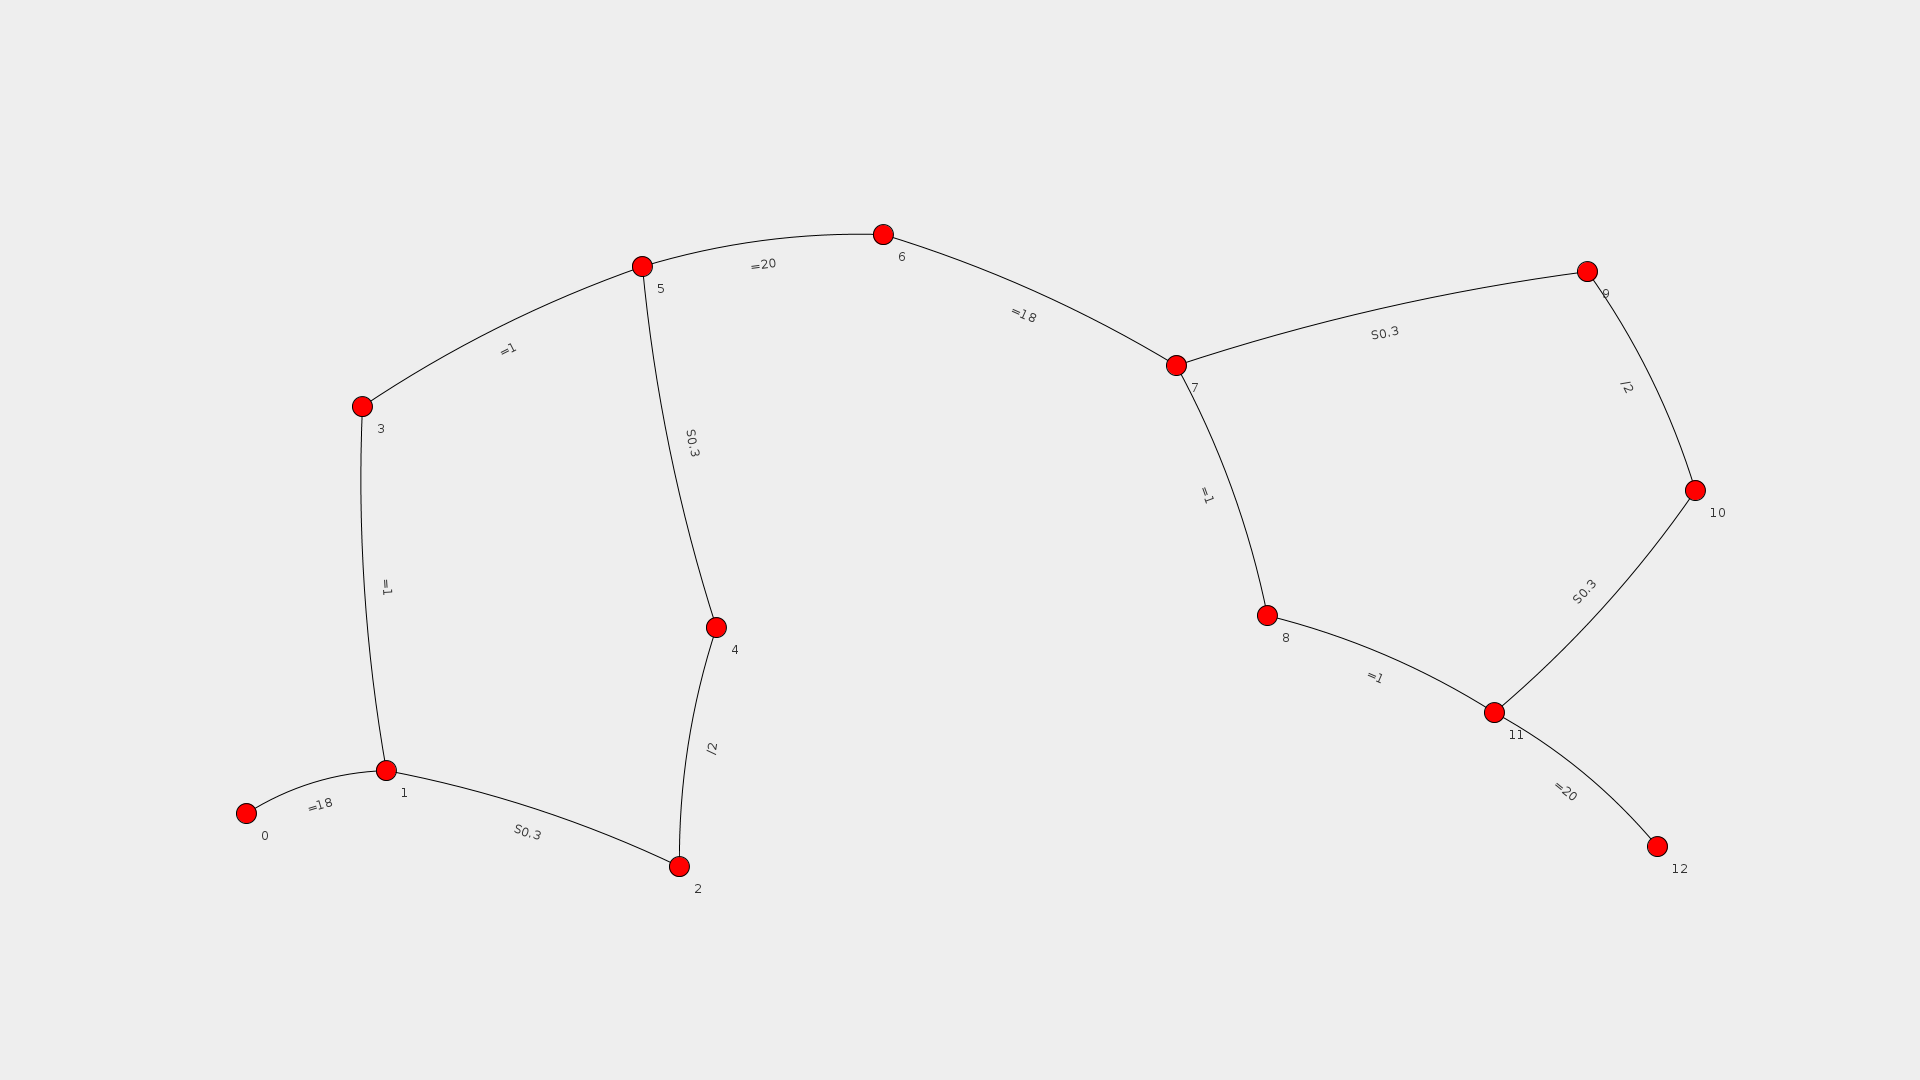
\includegraphics[width=150mm,angle=90]{solution.png}
\caption{RAS DATA SET TOY example territory. Undirected graph, arcs have descriptions.}
\end{figure}

\begin{figure}
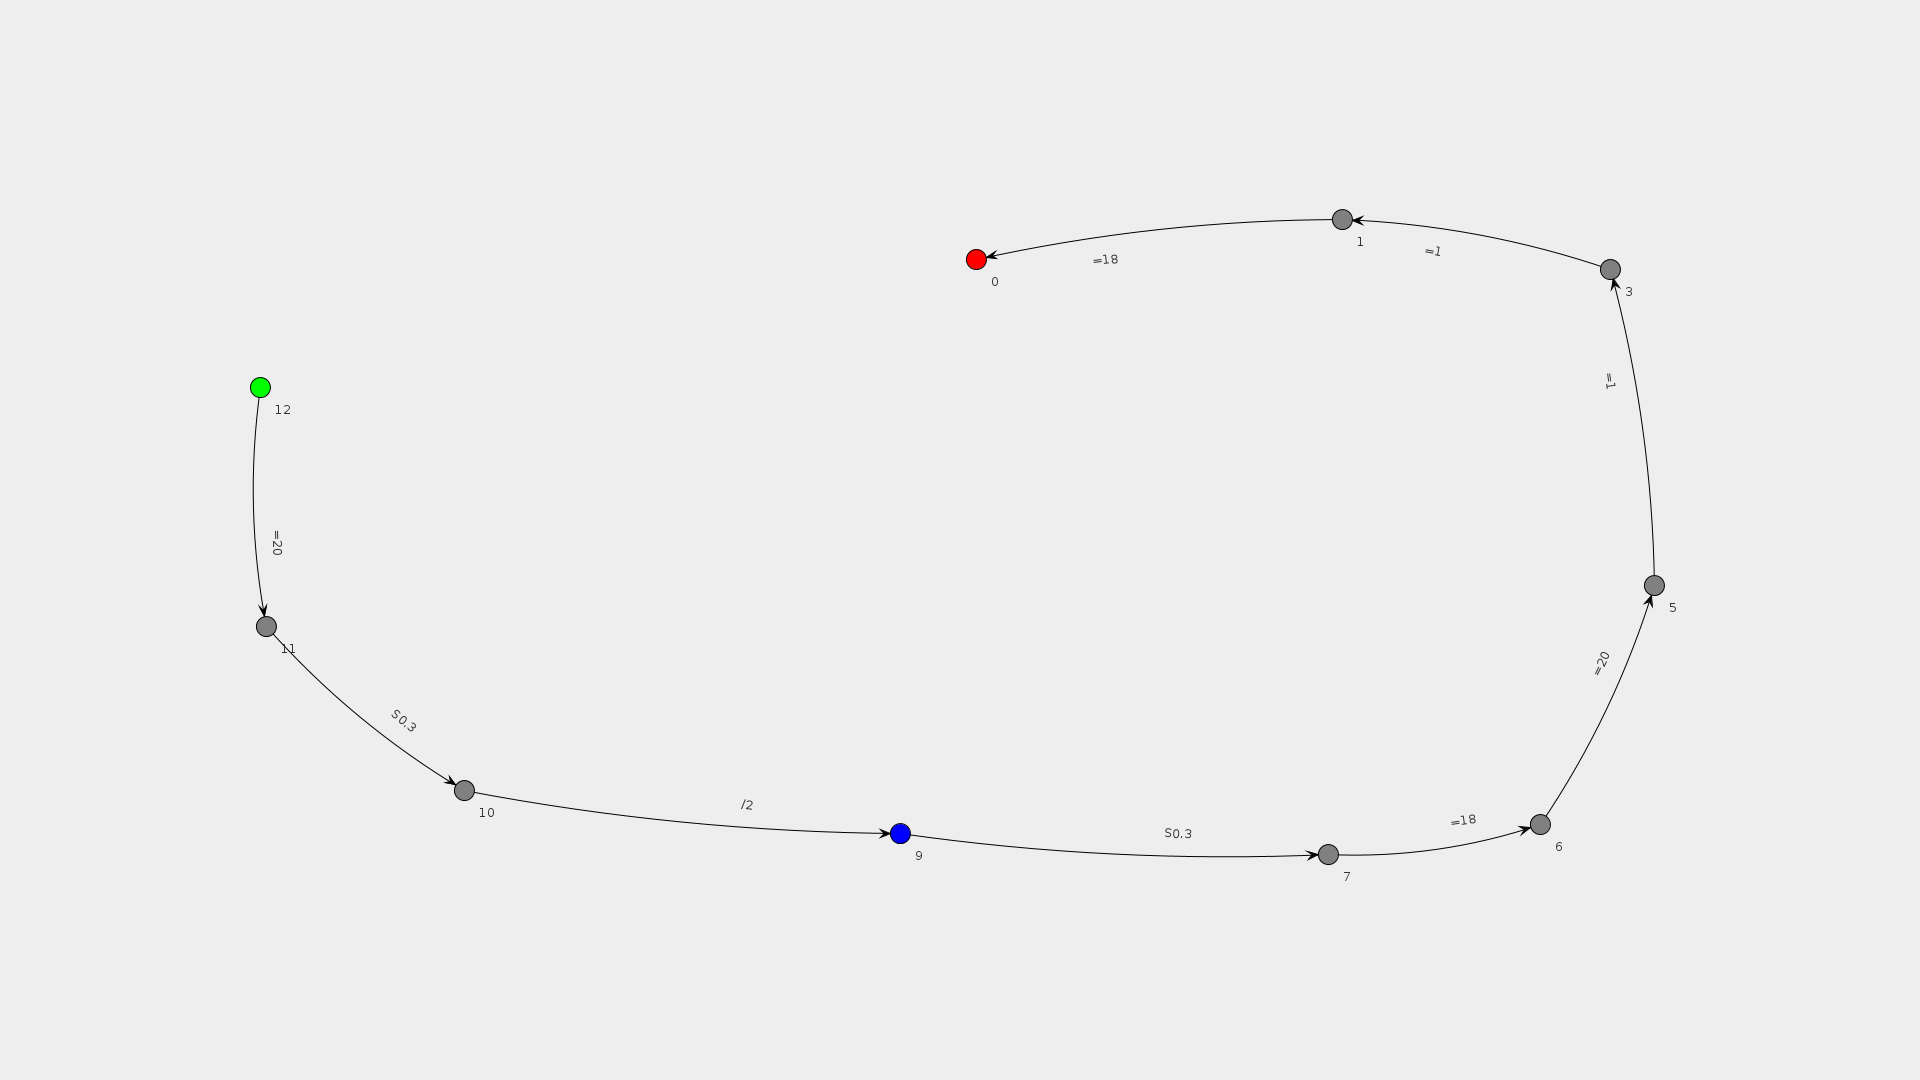
\includegraphics[width=150mm,angle=90]{B1.png}
\centering
\caption{RAS DATA SET TOY example, route of Train B1. Directed graph where green marks the origin, red the destination and blue is where the train is allowed to wait.}
\end{figure}

In this section, we show examples of visualizations that the solution is capable of providing. These visualizations have been rendered on the fly using the JUNG library\footnote{Java Universal Network/Graph framework, http://jung.sourceforge.net}.

\end{document}
